\section{Central Time-Of-Flight (CTOF)}

\subsection{Geometry}

The CLAS12 CTOF paddles and light guides are imported from the engineering model. The Step files are converted to tessellated STL files and imported
directly in the GEMC simulation \cite{gemcCad}. The STL files are downloaded using the coatjava geometry service, as the same files are used in reconstruction.
The paddles are assigned the scintillator material and associated with the ctof hit process routine.
The light guides are also associated to the scintillator material, but they are treated as passive material and not associated with a sensitive detector.

Each volume is typically tessellated by about 1,000 faucets. The simulation geometry captures complicated details such as the shape of the scintillator/light guides
junction, see \F{ctofGeometry} bottom.

\begin{figure}
	\centering
	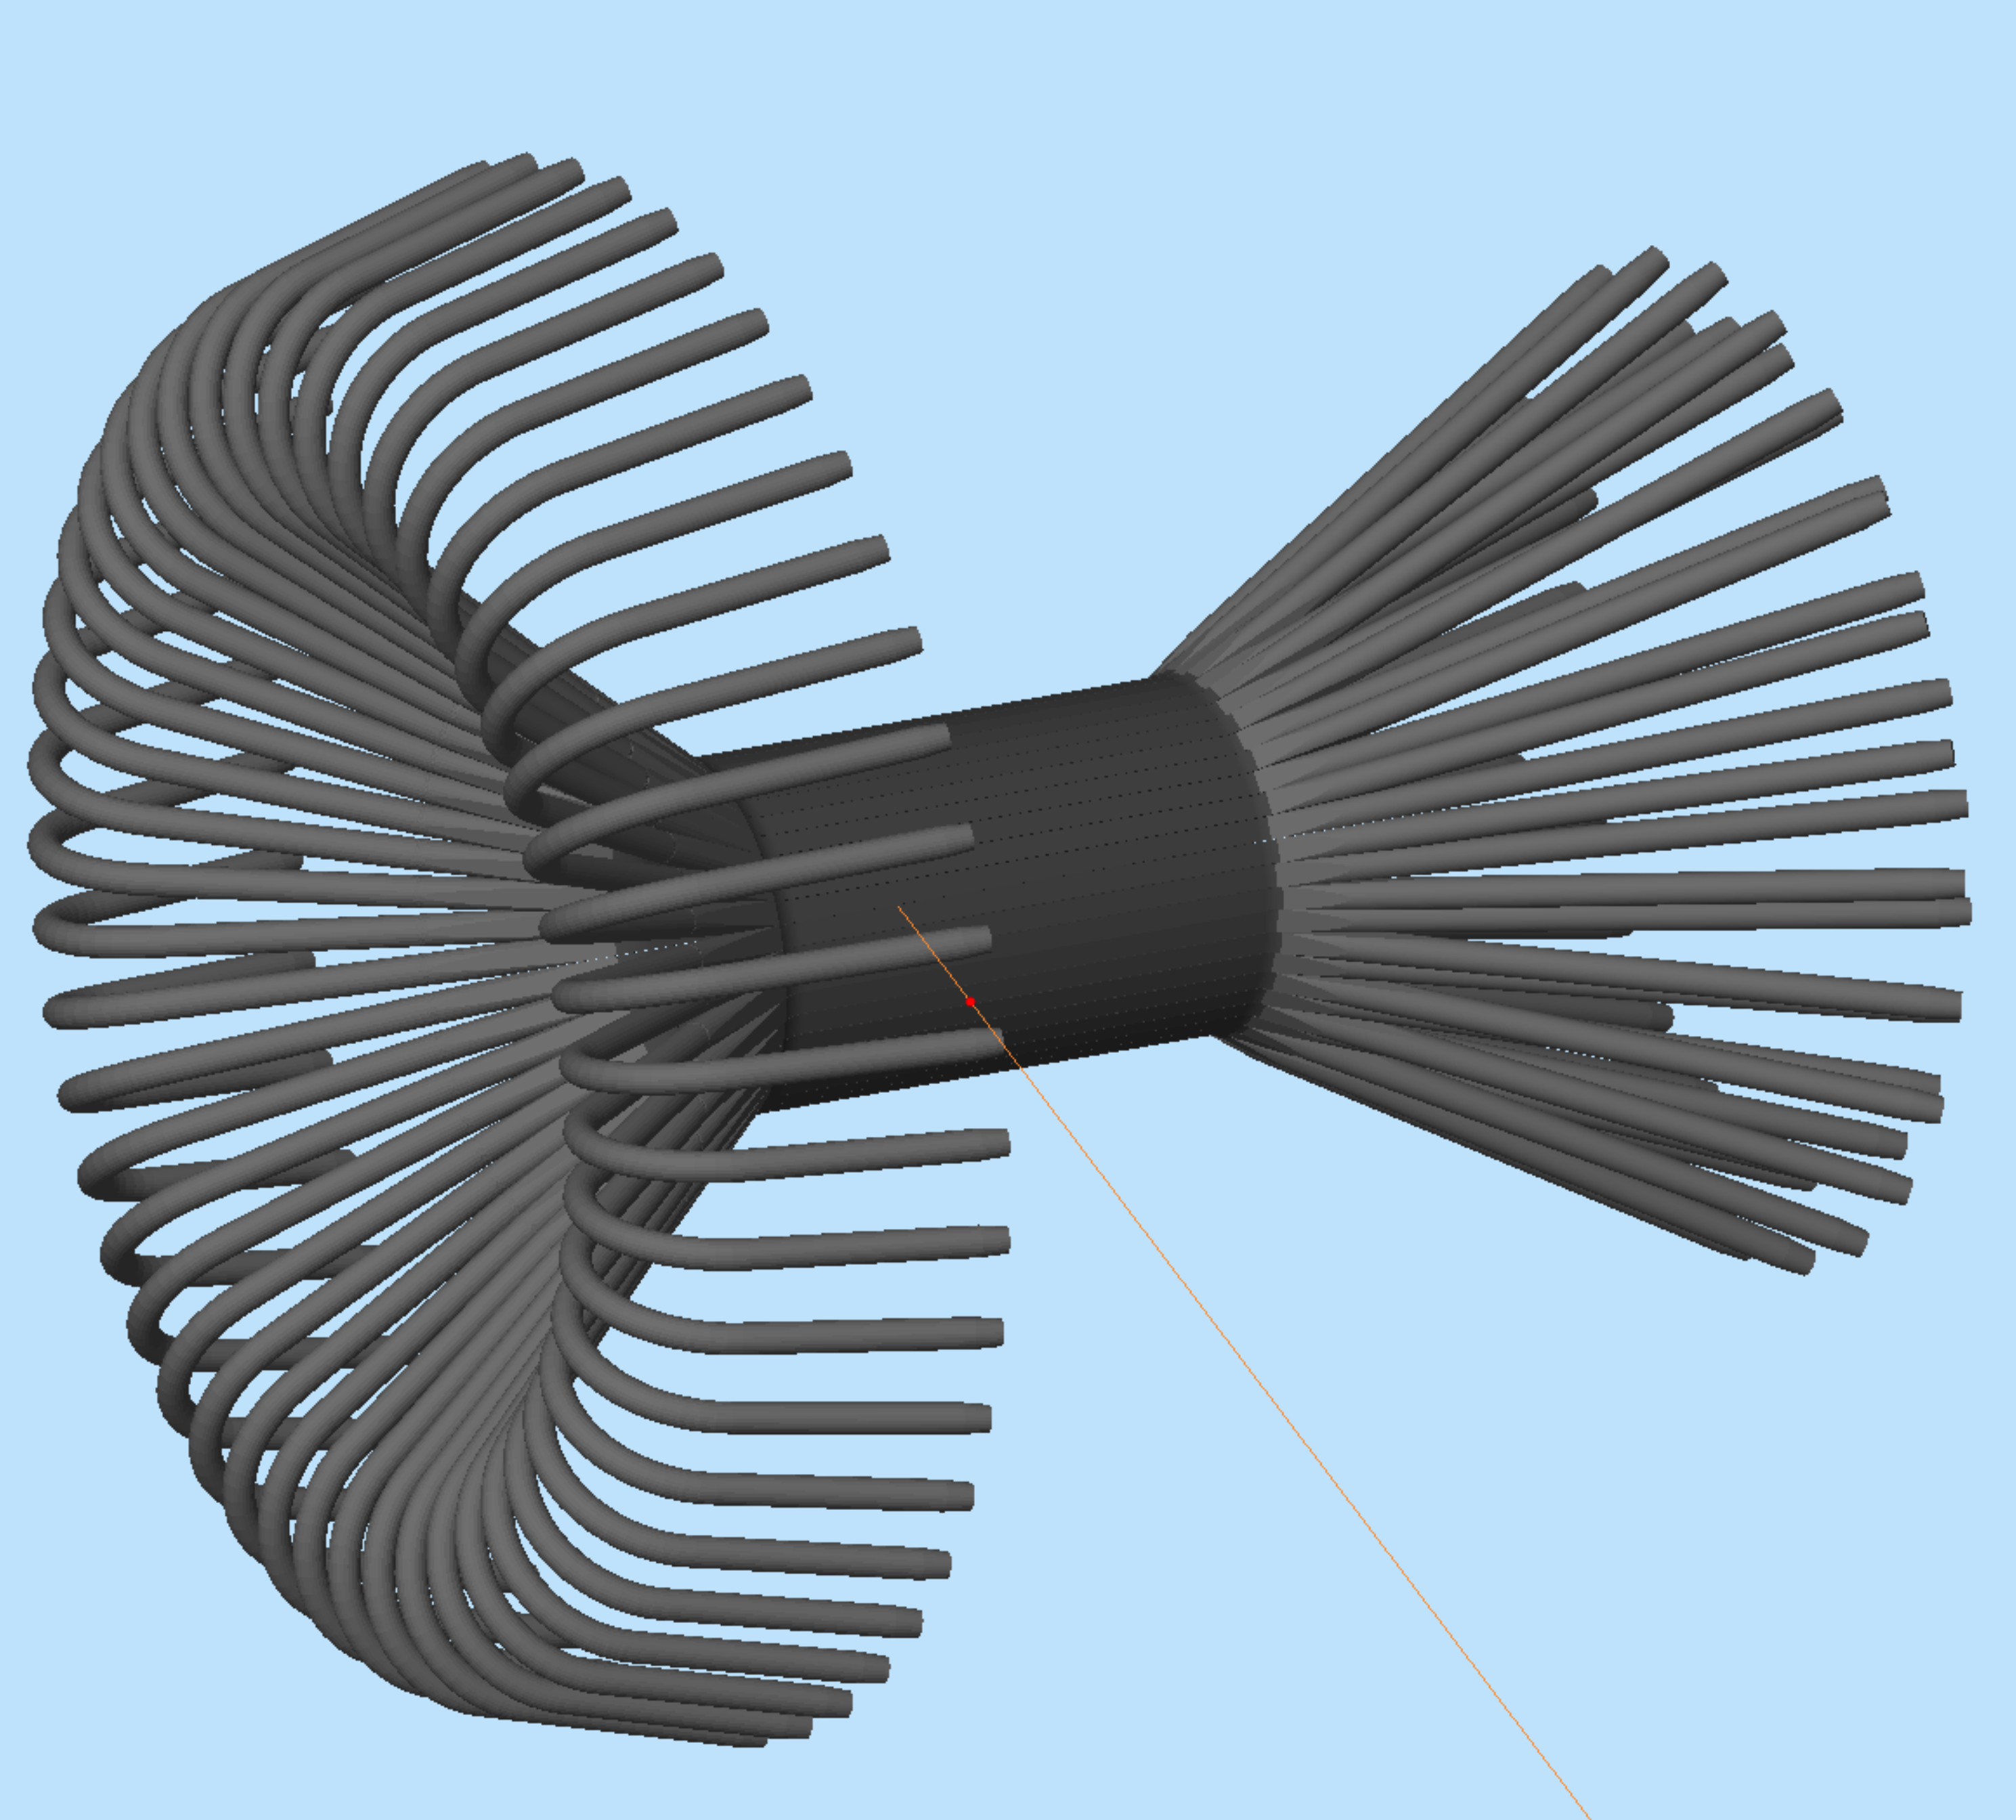
\includegraphics[width=0.95\columnwidth,keepaspectratio]{img/ctofGeometry.png}
	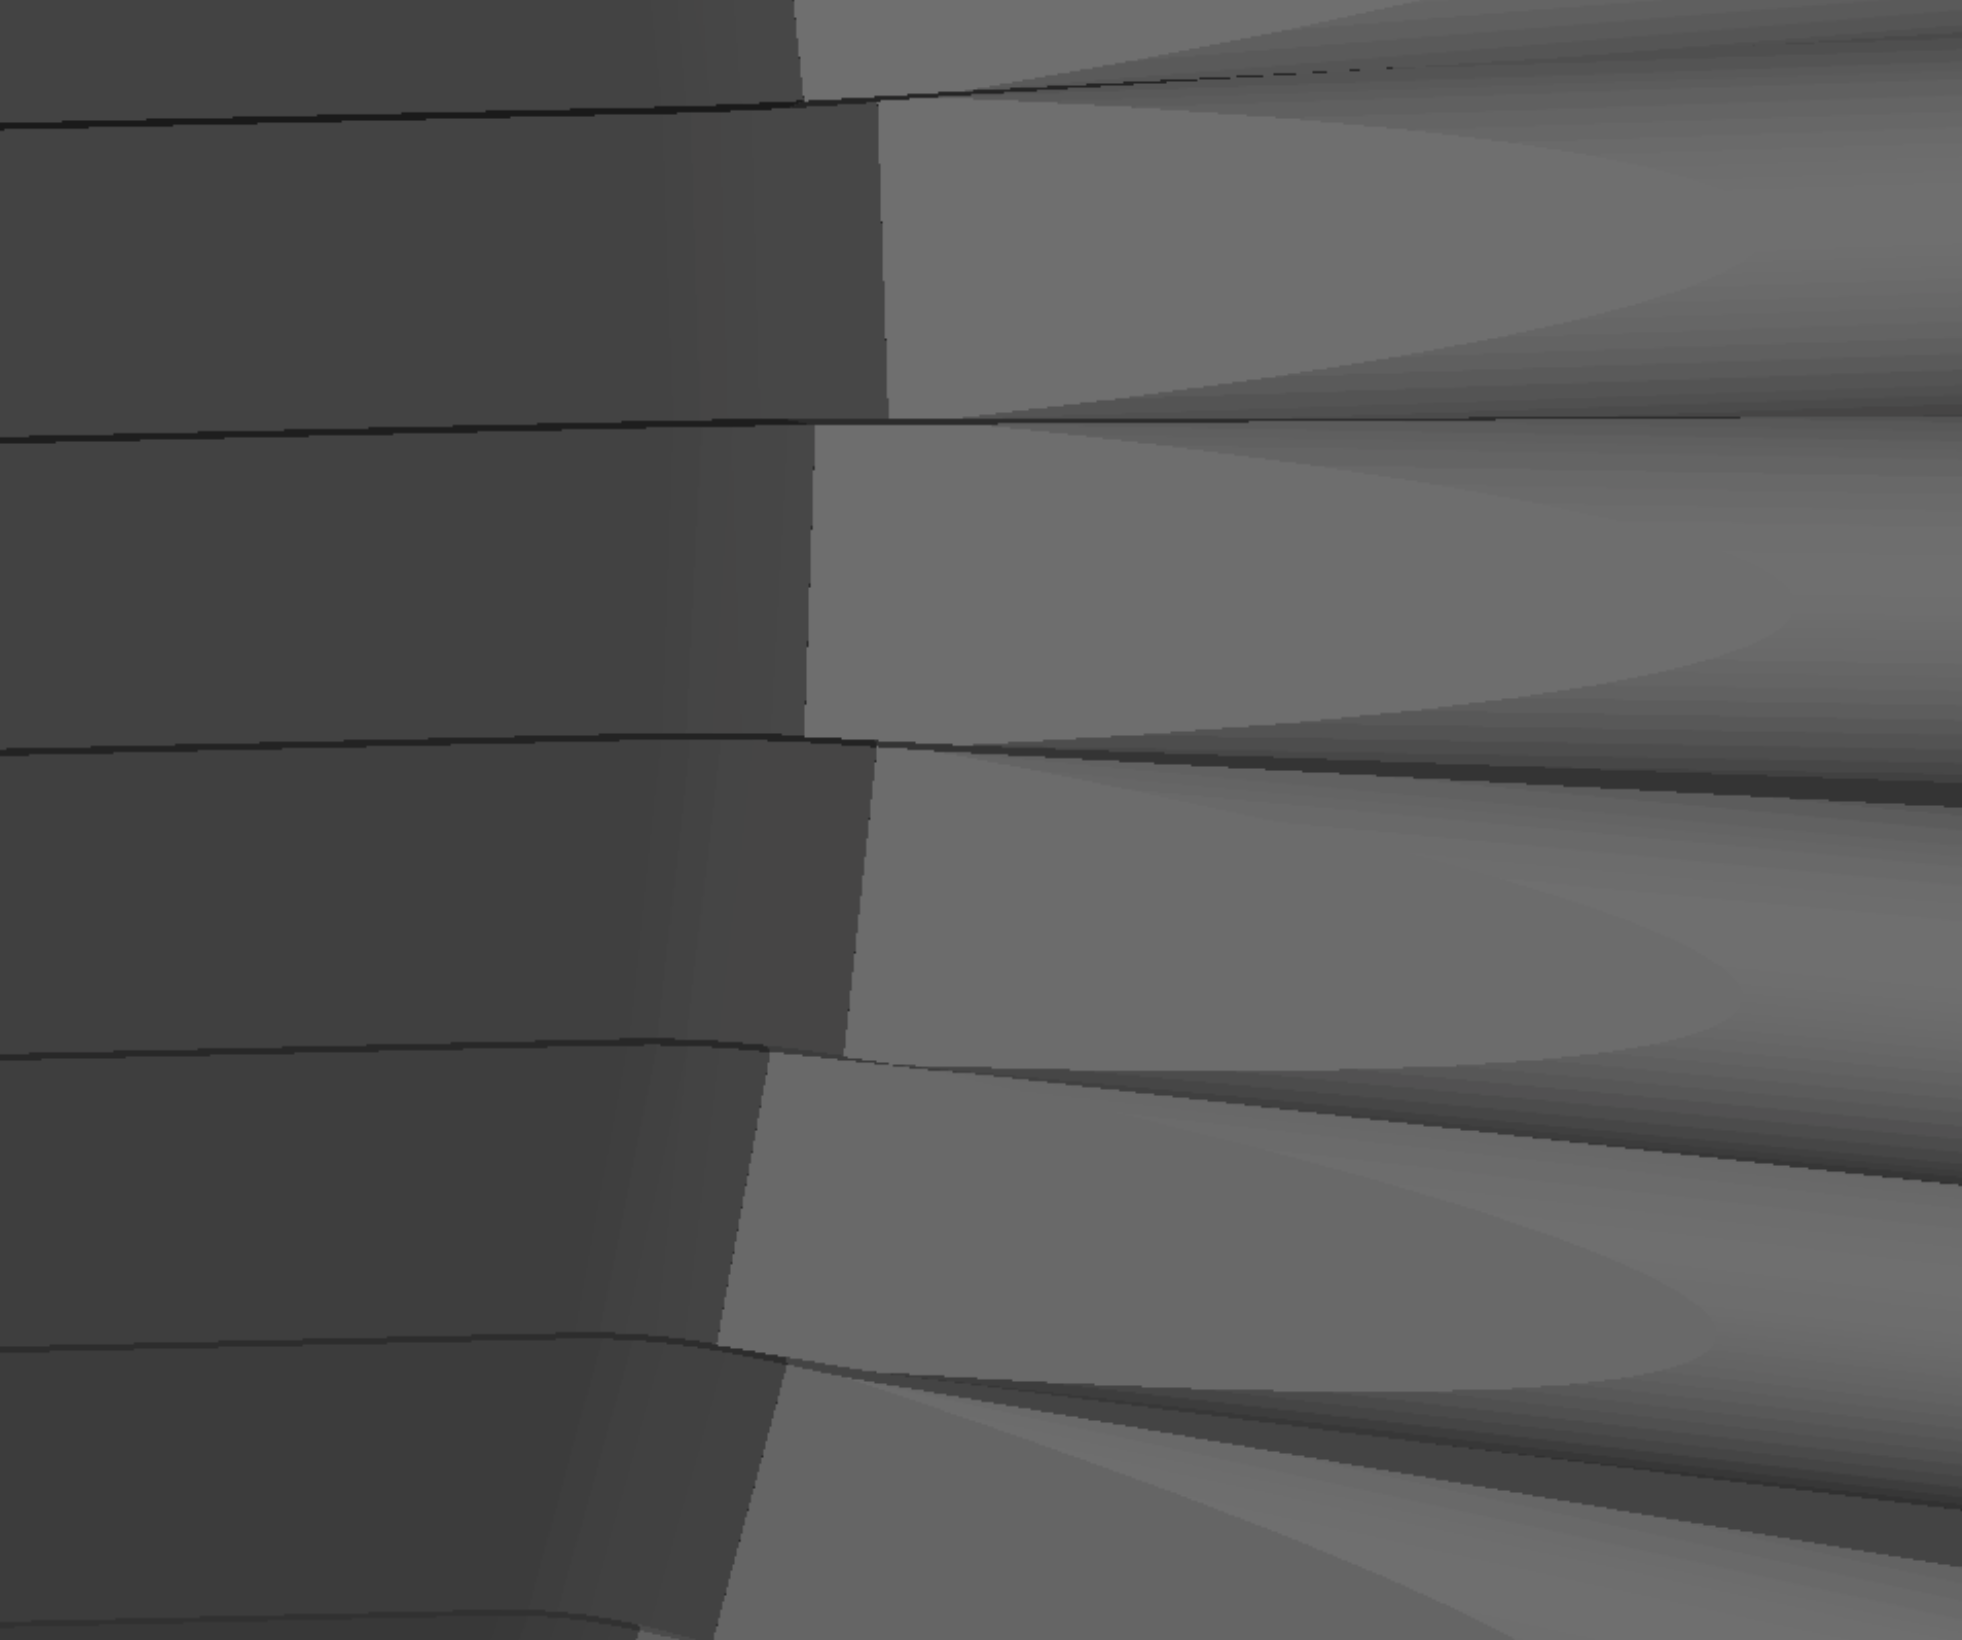
\includegraphics[width=0.95\columnwidth,keepaspectratio]{img/ctofDetail.png}
	\caption{Top: the GEMC implementation of the CTOF geometry. The paddles and light guides imported directly from the enginerring model.
			   The orange line shows a 2 GeV proton leaving a hit (red dot) in one of the paddles.
				Bottom: a zoom-in of the implementation shows the details of scintillator/light guides junction. }
	\label{fig:ctofGeometry}
\end{figure}


\subsubsection{Geometry Git Location}
The github location of the gemc perl api script is \url{https://github.com/gemc/detectors/tree/master/clas12/ctof}.
The coatjava geometry service is \url{https://github.com/JeffersonLab/clas12-offline-software/blob/development/common-tools/clas-jcsg/src/main/java/org/jlab/detector/geant4/v2/CTOFGeant4Factory.java}

\subsection{Process ID}

Each hit in the paddles is produces in two identical hits with the identifier variable "side" sets to 0 (for the left side PMT) and 1 (for right side PMT).
The hits are then processed independently through the ctof hit process routine.

\subsection{Digitization}

\subsubsection{ADC}

The energy deposited is reduced based on the position on the paddle using the calibration attenuation length. It is then corrected by a gain factor
to account for the fact that the HV are adjusted so that the geometeric mean sqrt(L*R) is independent of counter length.

The corrected energy is converted to the theoretical number of photos $N_{th}$ using the constant $500 \gamma / MeV $. A poissonian is used to
calculate the actual number of photons $N_{actual}$ and the resulting ``smeared`` energy is the converted to adc using the FADC conversion factor.


\subsubsection{TDC}

The absolute hit time is corrected by:

\begin{itemize}
	\item the effective velocity (from CCDB)
	\item the time walk correction, calculated from the smeared energy
	\item a panel to panel factor (from CCDB)
	\item a left/rigth time offset factor (from CCDB)
	\item an RF correction (from CCDB)
\end{itemize}

The time is then smeared by a $\sigma$ resolution read from CCDB using a gaussian function and then digitized using a TDC conversion factor.



\subsubsection{Summary of CCDB Table used}

\begin{itemize}
	\item /calibration/ctof/attenuation
	\item /calibration/ctof/effective\_velocity
	\item /calibration/ctof/status
	\item /calibration/ctof/gain\_balance
	\item /calibration/ctof/time\_walk
	\item /calibration/ctof/time\_offsets
	\item /calibration/ctof/tdc\_conv
	\item /geometry/ctof/ctof
	\item /daq/tt/ctof
\end{itemize}


\subsection{Digitized Bank}

The digitized output bank has $ID=400$, and the variables are summarized in Table \ref{tab:ctofBank}

\begin{table}[h]
	\begin{center}
		\begin{tabular}{| c | c | c |}
			\hline \hline
			Variable         & Description  & Tag  \\
			\hline
              sector  &                             sector number  &    1 \\
               layer  &               layer (1: 1A, 2: 1B, 3: 2B)  &    2 \\
              paddle  &                             paddle number  &    3 \\
                side  &                PMT side (0 Left, 1 Right)  &    4 \\
                 ADC  &                                       ADC  &    5 \\
                 TDC  &                                       TDC  &    6 \\
                ADCu  &                             ADC unsmeared  &    7 \\
                TDCu  &                             TDC unsmeared  &    8 \\
                hitn  &                                hit number  &   99 \\
			\hline \hline
		\end{tabular}
	\end{center}
	\caption{The digitized CTOF bank}\label{tab:ctofBank}
\end{table}


\subsubsection{Time Window}
The timewindow of the CTOF is set to 400 ns.

\subsubsection{Background merging algorithm}

\subsubsection{Process Routine Git Repository Location}
The CTOF hit process routine location in git is \url{https://github.com/gemc/source/blob/master/hitprocess/clas12/ctof_hitprocess.cc}
